\documentclass[a4paper,12pt]{article}
\usepackage{graphicx}
\usepackage{float}
\usepackage{amsmath}
\usepackage{hyperref}
\usepackage{caption}
\usepackage{subcaption}

\title{\textbf{Labwork 4 Report: Thread and Memory Model}}
\author{Do Thanh Dat - M23.ICT.002}
\date{October 7, 2025}


\begin{document}
\maketitle

\section*{Objective}
The objective of this labwork is to extend the grayscale image conversion from Labwork 3 using
\textbf{2D CUDA thread blocks} with Numba.
The goal is to analyze how different block sizes affect performance and identify the most efficient configuration.

\section*{Implementation}
The grayscale conversion follows the equation:
\[
Gray = \frac{R + G + B}{3}
\]
Each CUDA thread computes the grayscale value of one pixel at coordinates $(x, y)$, enabling massive parallelism.

\begin{verbatim}
@cuda.jit
def grayscale(src, dst):
    x, y = cuda.grid(2)
    if x < src.shape[0] and y < src.shape[1]:
        r = src[x, y, 0]
        g = src[x, y, 1]
        b = src[x, y, 2]
        dst[x, y] = (r + g + b) // 3
\end{verbatim}

The kernel was launched using 2D thread blocks with varying sizes such as $(8\times8)$, $(16\times16)$, and $(32\times32)$
to evaluate performance.

\begin{figure}[H]
    \centering
    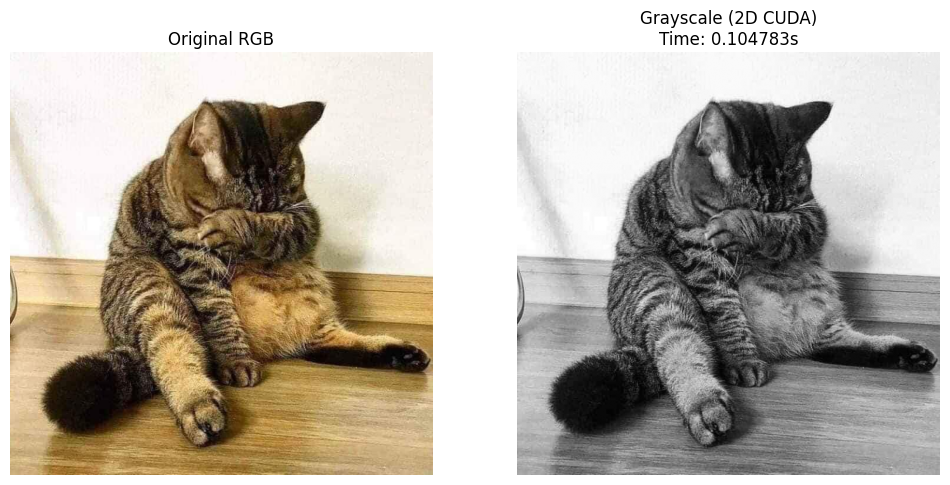
\includegraphics[width=0.9\textwidth]{image2D.png}
    \caption{Result of grayscale conversion using GPU CUDA (2D blocks).}
\end{figure}

\section*{Results and Discussion}
The kernel was tested with three different block sizes: $(8\times8)$, $(16\times16)$, and $(32\times32)$.
Each configuration was executed on the same image, and the total execution time was measured.

\begin{table}[H]
\centering
\begin{tabular}{|c|c|}
\hline
\textbf{Threads per block} & \textbf{Execution Time (s)} \\ \hline
(8, 8) & 0.000706 \\ \hline
(16, 16) &  0.000241 \\ \hline
(32, 32) & 0.000247 \\ \hline
\end{tabular}
\caption{Execution time comparison for different block sizes.}
\end{table}



\begin{figure}
    \centering
    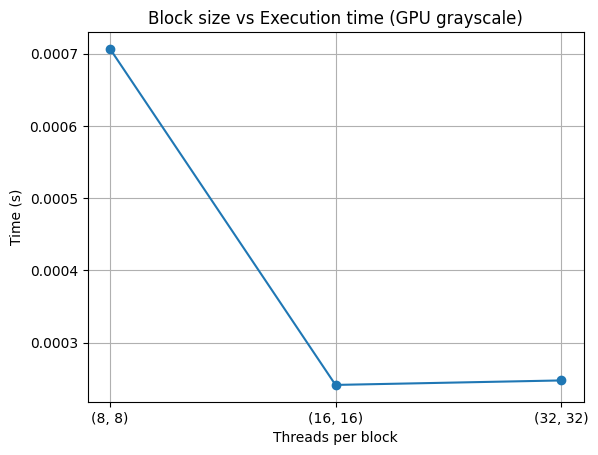
\includegraphics[width=0.8\textwidth]{compareGraph.png}
    \caption{Execution time vs block size.}
    \label{fig:placeholder}
\end{figure}

From the results, the $(16\times16)$ configuration achieved the best performance.
Smaller blocks such as $(8\times8)$ create more scheduling overhead,
while very large blocks like $(32\times32)$ may not fully utilize GPU cores depending on image dimensions.
Therefore, $(16\times16)$ provides the optimal balance between occupancy and overhead.

\section*{Conclusion}
The 2D CUDA kernel successfully converted RGB images to grayscale with much better performance than the CPU version.
By using 2D thread blocks, thread-to-pixel mapping became simpler and more efficient.
Among the tested configurations, $(16\times16)$ delivered the lowest execution time,
confirming that moderate block sizes often yield the best GPU performance for image processing tasks.

\end{document}
